\documentclass{article}

\usepackage{fancyhdr}
\usepackage{extramarks}
\usepackage{amsmath}
\usepackage{amsthm}
\usepackage{bm}
\usepackage{amsfonts}
\usepackage{tikz}
\usepackage[plain]{algorithm}
\usepackage{algpseudocode}
\usepackage{geometry}

\usetikzlibrary{automata,positioning}


%%%%%%%%%%%%%%%%%%%%%%%%%%%%%%%%%%%%%%%%%%%%%%%%%%%%%%%%%%%%%%%%%%%%%%%%%%%%%%%%%%%%%%%%%
% Basic Document Settings
%%%%%%%%%%%%%%%%%%%%%%%%%%%%%%%%%%%%%%%%%%%%%%%%%%%%%%%%%%%%%%%%%%%%%%%%%%%%%%%%%%%%%%%%%

%%% Page Size %%%
\geometry{
    a4paper,
    % total={170mm,257mm},
    % left=20mm,
    % top=20mm,
}
\voffset=0mm
\topmargin=-10mm
\textheight=245mm
\headsep=7mm
\footskip=11mm

\hoffset=0mm
\textwidth=159.2mm
\evensidemargin=0mm
\oddsidemargin=0mm

\linespread{1.1}
\setlength\parindent{0mm}
\setlength\parskip{10pt}
\allowdisplaybreaks

%%% Header & Footer %%%
\pagestyle{fancy}
% \lhead{\hmwkAuthorName}
\lhead{\hmwkClass\ \hmwkTitle}
% \rhead{\firstxmark}
\rhead{}
% \lfoot{\lastxmark}
\cfoot{Page | \thepage}
\renewcommand\headrulewidth{0.4pt}
\renewcommand\footrulewidth{0.4pt}

%%% Font %%%
\renewcommand{\familydefault}{\sfdefault}
% \renewcommand{\familydefault}{\rmdefault}


%%%%%%%%%%%%%%%%%%%%%%%%%%%%%%%%%%%%%%%%%%%%%%%%%%%%%%%%%%%%%%%%%%%%%%%%%%%%%%%%%%%%%%%%%
% Homework Details
%   - Title
%   - Due date
%   - Class
%   - Section/Time
%   - Instructor
%   - Author
%   - Updated Date
%%%%%%%%%%%%%%%%%%%%%%%%%%%%%%%%%%%%%%%%%%%%%%%%%%%%%%%%%%%%%%%%%%%%%%%%%%%%%%%%%%%%%%%%%
\newcommand{\hmwkTitle}{Assignment \#2 - Written Part}
\newcommand{\hmwkDueDate}{}
\newcommand{\hmwkClass}{Stanford CS224n (2023)}
\newcommand{\hmwkClassTime}{}
\newcommand{\hmwkClassInstructor}{}
\newcommand{\hmwkAuthorName}{\textbf{}}
\newcommand{\hmwkUpdateDate}{2\textsuperscript{nd} March, 2023}


%%%%%%%%%%%%%%%%%%%%%%%%%%%%%%%%%%%%%%%%%%%%%%%%%%%%%%%%%%%%%%%%%%%%%%%%%%%%%%%%%%%%%%%%%
% Title Page
%%%%%%%%%%%%%%%%%%%%%%%%%%%%%%%%%%%%%%%%%%%%%%%%%%%%%%%%%%%%%%%%%%%%%%%%%%%%%%%%%%%%%%%%%
\title{
    \vspace{2in}
    % \textmd{\textbf{\hmwkClass:\ \hmwkTitle}}\\
    % \normalsize\vspace{0.1in}\small{Due\ on\ \hmwkDueDate}\\
    \vspace{0.1in}\large{\textit{\hmwkClassInstructor\ \hmwkClassTime}}
    \vspace{3in}
}

\author{\hmwkAuthorName}
\date{}


%%%%%%%%%%%%%%%%%%%%%%%%%%%%%%%%%%%%%%%%%%%%%%%%%%%%%%%%%%%%%%%%%%%%%%%%%%%%%%%%%%%%%%%%%
% Create Problem Sections and Problem Environment
%
% This environment takes an optional argument. When given, it will adjust the
% problem counter. This is useful for when the problems given for your
% assignment aren't sequential. See the last 3 problems of this template for an
% example.
%%%%%%%%%%%%%%%%%%%%%%%%%%%%%%%%%%%%%%%%%%%%%%%%%%%%%%%%%%%%%%%%%%%%%%%%%%%%%%%%%%%%%%%%%
\newcommand{\hmwkSectionPrefix}{Question }
% \newcommand{\hmwkSectionPrefix}{Problem }

\newcommand{\hmwkSectionIndex}{\alph}
% \newcommand{\hmwkSectionIndex}{\arabic}

\newcommand{\hmwkSectionText}{\hmwkSectionPrefix (\hmwkSectionIndex{homeworkProblemCounter})}

\newcommand{\enterProblemHeader}[1]{
    \nobreak\extramarks{\hmwkSectionPrefix (\hmwkSectionIndex{#1}) continued on next page\ldots}\nobreak{}
    \nobreak\extramarks{\hmwkSectionPrefix (\hmwkSectionIndex{#1}) (continued)}{\hmwkSectionPrefix (\hmwkSectionIndex{#1}) continued on next page\ldots}\nobreak{}
}

\newcommand{\exitProblemHeader}[1]{
    \nobreak\extramarks{\hmwkSectionPrefix (\hmwkSectionIndex{#1}) (continued)}{\hmwkSectionPrefix (\hmwkSectionIndex{#1}) continued on next page\ldots}\nobreak{}
    \stepcounter{#1}
    \nobreak\extramarks{\hmwkSectionPrefix (\hmwkSectionIndex{#1})}{}\nobreak{}
}

\setcounter{secnumdepth}{0}
\newcounter{partCounter}
\newcounter{homeworkProblemCounter}
\setcounter{homeworkProblemCounter}{1}
\nobreak\extramarks{\hmwkSectionPrefix (\hmwkSectionIndex{homeworkProblemCounter})}{}\nobreak{}

\newenvironment{homeworkProblem}[1][-1]{
    \ifnum#1>0
        \setcounter{homeworkProblemCounter}{#1}
    \fi
    \section{\hmwkSectionText}
    \setcounter{partCounter}{1}
    \enterProblemHeader{homeworkProblemCounter}
}{
    \exitProblemHeader{homeworkProblemCounter}
}


%%%%%%%%%%%%%%%%%%%%%%%%%%%%%%%%%%%%%%%%%%%%%%%%%%%%%%%%%%%%%%%%%%%%%%%%%%%%%%%%%%%%%%%%%
% Various Helper Commands
%%%%%%%%%%%%%%%%%%%%%%%%%%%%%%%%%%%%%%%%%%%%%%%%%%%%%%%%%%%%%%%%%%%%%%%%%%%%%%%%%%%%%%%%%
\renewcommand{\part}[1]{\textbf{Part \alph{partCounter}}\stepcounter{partCounter}\\}

% Useful for algorithms
\newcommand{\alg}[1]{\textsc{\bfseries \footnotesize #1}}

% For derivatives
\newcommand{\deriv}[1]{\frac{\mathrm{d}}{\mathrm{d}x} (#1)}

% For partial derivatives
\newcommand{\pderiv}[2]{\frac{\partial}{\partial #1} (#2)}

% Integral dx
\newcommand{\dx}{\mathrm{d}x}

% Alias for the Solution section header
\newcommand{\solution}{\textbf{\large Solution}}

% Probability commands: Expectation, Variance, Covariance, Bias
\newcommand{\E}{\mathrm{E}}
\newcommand{\Var}{\mathrm{Var}}
\newcommand{\Cov}{\mathrm{Cov}}
\newcommand{\Bias}{\mathrm{Bias}}


%%%%%%%%%%%%%%%%%%%%%%%%%%%%%%%%%%%%%%%%%%%%%%%%%%%%%%%%%%%%%%%%%%%%%%%%%%%%%%%%%%%%%%%%%
% Main Document
%%%%%%%%%%%%%%%%%%%%%%%%%%%%%%%%%%%%%%%%%%%%%%%%%%%%%%%%%%%%%%%%%%%%%%%%%%%%%%%%%%%%%%%%%
\begin{document}
% \maketitle
% \pagebreak
{Updated on: \hmwkUpdateDate}
\begin{homeworkProblem}

    Note that
    \[
        \bm{y}_w = \begin{cases}
                        1 &\text{if } w = o \\
                        0 &\text{if } w \neq o
                    \end{cases}
    \]
    Therefore,
    \begin{align*}
        -\sum_{w \in \text{Vocab}} \bm{y}_w \log{(\bm{\hat{y}}_w)}
            &= - (1) \log{(\bm{\hat{y}_o})} \\
            &= - \log{(\bm{\hat{y}_o})}
    \end{align*}
\end{homeworkProblem}


\begin{homeworkProblem}
    \textbf{Part (i)}
    \begin{align*}
        J_{naive-softmax}(\bm{v}_c, o, \bm{U})
        &= - \log{(\bm{\hat{y}_o})} \\
        &= - \log{\left(
            \frac{\exp{(\bm{u}_o^\top\bm{v_c})}}
                {\sum_{k\in\text{|Vocab|}} \exp{(\bm{u}_k^\top\bm{v_c})}}
        \right)} \\
        &= - \log{\left(\exp{(\bm{u}_o^\top\bm{v_c})}\right)} + \log{\left(\sum_{k\in\text{|Vocab|}}\exp{(\bm{u}_k^\top\bm{v_c})}\right)}\\
        &= - \bm{u}_o^\top\bm{v_c} + \log{\left(\sum_{k\in\text{|Vocab|}}\exp{(\bm{u}_k^\top\bm{v_c})}\right)}\\\\
        \frac{\partial J_{naive-softmax}(\bm{v}_c, o, \bm{U})}{\partial \bm{v_c}}
        &= \frac{\partial}{\partial \bm{v_c}}\left[-\bm{u}_o^\top\bm{v_c} + \log{\left(\sum_{k\in\text{|Vocab|}}\exp{(\bm{u}_k^\top\bm{v_c})}\right)}\right]\\
        &= -\bm{u_o} + \frac{\sum_{k\in\text{|Vocab|}}\exp{(\bm{u}_k^\top\bm{v_c})}\bm{u_k}}{\sum_{k\in\text{|Vocab|}}\exp{(\bm{u}_k^\top\bm{v_c})}}\\
        &= -\bm{u_o} + \sum_{k\in\text{|Vocab|}} \left(\frac{\exp{(\bm{u}_k^\top\bm{v_c})}}{\sum_{k\in\text{|Vocab|}}\exp{(\bm{u}_k^\top\bm{v_c})}}\right)\bm{u_k} \\
        &= -\bm{u_o} + \sum_{k\in\text{|Vocab|}} \left(\bm{\hat{y}_k}\right)\bm{u_k}\\
        &= \sum_{k\in\text{|Vocab|}} \bm{y_k}(-\bm{u_k}) + \sum_{k\in\text{|Vocab|}} \left(\bm{\hat{y}_k}\right)\bm{u_k}\\
        &= \sum_{k\in\text{|Vocab|}} \left(\bm{\hat{y}_k} - \bm{y_k}\right) \bm{u_k} \\
        &= (\bm{\hat{y}^\top} - \bm{y^\top}) \bm{U^\top} \qquad (\text{a row vector})\\
        &= \bm{U} (\bm{\hat{y}} - \bm{y}) \qquad (\text{a colume vector})
    \end{align*}
    Note that a column vector is left as the answer to follow the shape convention.

    \vspace{1em}

    \textbf{Part (ii)}

    If the gradient computed in (b)(i) is equal to zero, i.e. the equation $\bm{U}(\bm{\hat{y}}-\bm{y})=0$ is satisfied, then the vector $(\bm{\hat{y}}-\bm{y})$ lies in the nullspace of the matrix $\bm{U}$. Since the zero vector is always in the nullspace, a trival solution to the equation is $\bm{\hat{y}}-\bm{y}=0$, i.e. the predicted word vector is correct.

    \vspace{1em}

    \textbf{Part (iii)}
    \begin{align*}
        \frac{\partial J_{naive-softmax}(\bm{v}_c, o, \bm{U})}{\partial \bm{v_c}}
        &= \bm{U} (\bm{\hat{y}} - \bm{y})\\
        &= \bm{U} \bm{\hat{y}} - \bm{U} \bm{y}\\
        &= \text{predicted word vector} - \text{true word vector}
    \end{align*}
    When the gradient is subtractedf from the word vecter $\bm{v_c}$ , $\bm{v_c}$ is improved towards the true word vector since the true word vector is added to $\bm{v_c}$. On the other hand, the updated vector is moved away from the predicted word vector since the predicted word vector is subtracted from $\bm{v_c}$.

    \vspace{1em}

    \textbf{Part (iv)}

    Consider two word vectors $\mathbf{u_x}$ and $\mathbf{u_y}$ of the two different words $\mathbf{x}$ and $\mathbf{y}$, where $\mathbf{u_x}=\alpha\mathbf{u_y}$ and $\alpha$ is some scalar.

    If the two words are opposite in meanings, it is expected that these two word vectors are in opposite direction, i.e. $\alpha<0$. In such case, since the L2 normalization preserves the direction of the word vectors, one can still distinguish the two word vectors with their directions.

    In the case where the two words have the same sign ($\alpha>0$) but with different extent (e.g. $\mathbf{x}$ is much positive than $\mathbf{y}$), one would expect such information is revealed from the vector magnitudes. However, the L2 normalization produces vectors with the same magnitudes. Information of word vectors carried by the vector magnitude is lost after performing L2 normalization.
\end{homeworkProblem}


\begin{homeworkProblem}
    \[
        J_{naive-softmax}(\boldsymbol{v}_c, o, \boldsymbol{U})
        = - \boldsymbol{u}_o^\top\boldsymbol{v_c} + \log{\left(\sum_{k\in\text{|Vocab|}}\exp{(\boldsymbol{u}_k^\top\boldsymbol{v_c})}\right)}
    \]
    When $w \neq o$,
    \begin{align*}
        \frac{\partial J_{naive-softmax}(\boldsymbol{v}_c, o, \boldsymbol{U})}{\partial \boldsymbol{u_{w\neq o}}}
        &= \frac{\partial}{\partial \boldsymbol{u_{w\neq o}}}\left[-\boldsymbol{u}_o^\top\boldsymbol{v_c} + \log{\left(\sum_{k\in\text{|Vocab|}}\exp{(\boldsymbol{u}_k^\top\boldsymbol{v_c})}\right)}\right] \\
        &= 0 + \frac{\exp{(\boldsymbol{u}_{w\neq o}^\top\boldsymbol{v_c})}\boldsymbol{v_c}}{\sum_{k\in\text{|Vocab|}}\exp{(\boldsymbol{u}_k^\top\boldsymbol{v_c})}}\\
        &= \left(\frac{\exp{(\boldsymbol{u}_{w\neq o}^\top\boldsymbol{v_c})}}{\sum_{k\in\text{|Vocab|}}\exp{(\boldsymbol{u}_k^\top\boldsymbol{v_c})}}\right) \boldsymbol{v_c}\\
        &= \boldsymbol{\hat{y}_{w\neq o}} \boldsymbol{v_c}\\
    \end{align*}

    When $w = o$,
    \begin{align*}
        \frac{\partial J_{naive-softmax}(\boldsymbol{v}_c, o, \boldsymbol{U})}{\partial \boldsymbol{u_{w = o}}}
        &= \frac{\partial}{\partial \boldsymbol{u_{w=o}}}\left[-\boldsymbol{u}_o^\top\boldsymbol{v_c} + \log{\left(\sum_{k\in\text{|Vocab|}}\exp{(\boldsymbol{u}_k^\top\boldsymbol{v_c})}\right)}\right] \\
        &= -\boldsymbol{v_c} + \frac{\exp{(\boldsymbol{u}_{w= o}^\top\boldsymbol{v_c})}\boldsymbol{v_c}}{\sum_{k\in\text{|Vocab|}}\exp{(\boldsymbol{u}_k^\top\boldsymbol{v_c})}}\\
        &= -\boldsymbol{v_c} + \left(\frac{\exp{(\boldsymbol{u}_{w= o}^\top\boldsymbol{v_c})}}{\sum_{k\in\text{|Vocab|}}\exp{(\boldsymbol{u}_k^\top\boldsymbol{v_c})}}\right) \boldsymbol{v_c}\\
        &= -\boldsymbol{v_c} + \boldsymbol{\hat{y}_{w= o}} \boldsymbol{v_c}\\
        &= (\boldsymbol{\hat{y}_{w=o}}-1) \boldsymbol{v_c}
    \end{align*}
    Therefore,
    \[
        \frac{\partial J_{naive-softmax}(\boldsymbol{v}_c, o, \boldsymbol{U})}{\partial \boldsymbol{u_w}} =
        \begin{cases}
        \boldsymbol{\hat{y}_{w}} \boldsymbol{v_c}     &\text{if } w \neq o \\
        (\boldsymbol{\hat{y}_{w}}-1) \boldsymbol{v_c} &\text{if } w = o
        \end{cases}
    \]
\end{homeworkProblem}


\begin{homeworkProblem}
    \[
        \frac{\partial J_{naive-softmax}(\boldsymbol{v}_c, o, \boldsymbol{U})}{\partial \boldsymbol{U}} =
            \begin{pmatrix}
                \frac{\partial J(\boldsymbol{v}_c, o, \boldsymbol{U})}{\partial \boldsymbol{u_1}} &
                \frac{\partial J(\boldsymbol{v}_c, o, \boldsymbol{U})}{\partial \boldsymbol{u_2}} &
                ... &
                \frac{\partial J(\boldsymbol{v}_c, o, \boldsymbol{U})}{\partial \boldsymbol{u_{|\text{Vocab}|}}}
            \end{pmatrix}
    \]
\end{homeworkProblem}


\begin{homeworkProblem}
    \begin{align*}
        f(x) &= \max(\alpha x, x) \\
            &= \begin{cases}
                    \alpha x &\text{if }  x < 0 \\
                    x        &\text{if } x > 0
                \end{cases}\\
        \frac{df(x)}{dx} &= \begin{cases}
                                \alpha &\text{if }  x < 0 \\
                                1      &\text{if } x > 0
                            \end{cases}
    \end{align*}
\end{homeworkProblem}


\begin{homeworkProblem}
    \begin{align*}
        \frac{d}{dx} \sigma(x) &= \frac{d}{dx} \left( \frac{e^x}{e^x+1}\right) \\
                               &= \frac{e^x}{e^x+1} - \frac{e^{2x}}{(e^x+1)^2} \\
                               &= \sigma(x) - \sigma(x)^2 \\
                               &= \sigma(x) \left( 1 - \sigma(x) \right) \\
     \end{align*}
\end{homeworkProblem}

\pagebreak

\begin{homeworkProblem}
    \textbf{Part (i)}
    \begin{align*}
        \frac{d}{dx} \log \sigma(x) &= \frac{1}{\sigma(x)} \left( \frac{d}{dx} \sigma(x) \right) \\
        &= \frac{1}{\sigma(x)} \left( \sigma(x) \left( 1 - \sigma(x) \right) \right) \\
        &= 1 - \sigma(x)
    \end{align*}
    \[
        J_{\text{negative-sample}}(\boldsymbol{v}_c, o, \boldsymbol{U}) = - \log (\sigma(\boldsymbol{u}_o^\top\boldsymbol{v_c})) - \sum_{s=1}^{K} \log (\sigma(-\boldsymbol{u}_{w_s}^\top\boldsymbol{v_c}))
    \]
    \begin{align*}
        \frac{\partial J_{\text{negative-sample}}(\boldsymbol{v}_c, o, \boldsymbol{U})}{\partial \boldsymbol{v_c}}
        &= (\sigma(\boldsymbol{u}_o^\top\boldsymbol{v_c}) - 1) \frac{\partial}{\partial \boldsymbol{v_c}} (\boldsymbol{u}_o^\top\boldsymbol{v_c})
            + \sum_{s=1}^{K} (\sigma(-\boldsymbol{u}_{w_s}^\top\boldsymbol{v_c}) - 1) \frac{\partial}{\partial \boldsymbol{v_c}} (-\boldsymbol{u}_{w_s}^\top\boldsymbol{v_c}) \\
        &= (\sigma(\boldsymbol{u}_o^\top\boldsymbol{v_c}) - 1) \boldsymbol{u}_o
            - \sum_{s=1}^{K} (\sigma(-\boldsymbol{u}_{w_s}^\top\boldsymbol{v_c}) - 1) \boldsymbol{u}_{w_s} \\
        \\
        \frac{\partial J_{\text{negative-sample}}(\boldsymbol{v}_c, o, \boldsymbol{U})}{\partial \boldsymbol{u_o}}
        &= (\sigma(\boldsymbol{u}_o^\top\boldsymbol{v_c}) - 1) \frac{\partial}{\partial \boldsymbol{u_o}} (\boldsymbol{u}_o^\top\boldsymbol{v_c})
            + 0\\
        &= (\sigma(\boldsymbol{u}_o^\top\boldsymbol{v_c}) - 1) \boldsymbol{v}_c \\
        \\
        \frac{\partial J_{\text{negative-sample}}(\boldsymbol{v}_c, o, \boldsymbol{U})}{\partial \boldsymbol{u_{w_s}}}
        &= 0 + (\sigma(-\boldsymbol{u}_{w_s}^\top\boldsymbol{v_c}) - 1) \frac{\partial}{\partial \boldsymbol{u_{w_s}}} (-\boldsymbol{u}_{w_s}^\top\boldsymbol{v_c}) \\
        &= - (\sigma(-\boldsymbol{u}_{w_s}^\top\boldsymbol{v_c}) - 1) \boldsymbol{v}_c
    \end{align*}

    \vspace{1em}

    \textbf{Part (ii)}
    \[
        \boldsymbol{U_{o,\{w_1, ...,w_K\}}} = \left[ \boldsymbol{u_o},  -\boldsymbol{u_{w_1}}, \cdots, -\boldsymbol{u_{w_K}} \right]
    \]
    Denote
    \begin{align*}
        \boldsymbol{\lambda} &= \sigma \left( \boldsymbol{U_{o,\{w_1, \cdots,w_K\}}^\top}\boldsymbol{v_c} \right) - \boldsymbol{1} \\
        &= \begin{pmatrix}
                \sigma(\boldsymbol{u}_o^\top\boldsymbol{v_c}) - 1\\
                \sigma(-\boldsymbol{u}_{w_1}^\top\boldsymbol{v_c}) - 1\\
                \vdots\\
                \sigma(-\boldsymbol{u}_{w_K}^\top\boldsymbol{v_c}) - 1\\
            \end{pmatrix}\\
        &= \begin{pmatrix}
                \lambda_o\\
                \lambda_1\\
                \vdots\\
                \lambda_K\\
            \end{pmatrix}
    \end{align*}
    Each element of $\boldsymbol{\lambda}$ is used in computing the partial derivatives in part (g)(i). The derivatives are simplified as follows:
    \begin{align*}
        \frac{\partial J_{\text{negative-sample}}(\boldsymbol{v}_c, o, \boldsymbol{U})}{\partial \boldsymbol{v_c}}
        &= \lambda_o \boldsymbol{u}_o
            - \sum_{s=1}^{K} \lambda_s \boldsymbol{u}_{w_s} \\
        \frac{\partial J_{\text{negative-sample}}(\boldsymbol{v}_c, o, \boldsymbol{U})}{\partial \boldsymbol{u_o}}
        &= \lambda_o \boldsymbol{v}_c \\
        \frac{\partial J_{\text{negative-sample}}(\boldsymbol{v}_c, o, \boldsymbol{U})}{\partial \boldsymbol{u_{w_s}}}
        &= - \lambda_s \boldsymbol{v}_c
    \end{align*}

    \pagebreak

    \textbf{Part (iii)}

    The computation of $J_{\text{naive-softmax}}$ requires computing the dot products between all word vectors with the input vector. The time complexity of the computation is $O(|\text{Vocab}|)$. On the other hand, the computation of $J_{\text{negative-sample}}$ involves only the dot products between K negative sample word vectors and the input vectors, where the time complexity of computation is $O(K)$. Hence, computing the negative sampling loss function is much more efficient than the naive-softmax function.

\end{homeworkProblem}


\begin{homeworkProblem}
    \begin{align*}
        \frac{\partial J_{\text{negative-sample}}(\boldsymbol{v}_c, o, \boldsymbol{U})}{\partial \boldsymbol{u_{w_s}}}
        &= \frac{\partial}{\partial \boldsymbol{u_{w_s}}}
            \left( - \log (\sigma(\boldsymbol{u}_o^\top\boldsymbol{v_c}))
                    - \sum_{k=1}^{K} \log (\sigma(-\boldsymbol{u}_{w_k}^\top\boldsymbol{v_c}))
            \right)\\
        &= \frac{\partial}{\partial \boldsymbol{u_{w_s}}}
            \left( - \log (\sigma(\boldsymbol{u}_o^\top\boldsymbol{v_c}))
                    - \sum_{\substack{k=1 \\ w_k \neq w_s}}^{K} \log (\sigma(-\boldsymbol{u}_{w_k}^\top\boldsymbol{v_c}))
                    - \sum_{\substack{k=1 \\ w_k = w_s}}^{K} \log (\sigma(-\boldsymbol{u}_{w_k}^\top\boldsymbol{v_c}))
            \right)\\
        &= 0
            - 0 -
            \frac{\partial}{\partial \boldsymbol{u_{w_s}}}
            \left(
                    \sum_{\substack{k=1 \\ w_k = w_s}}^{K} \log (\sigma(-\boldsymbol{u}_{w_k}^\top\boldsymbol{v_c}))
            \right)\\
        &= - \sum_{\substack{k=1 \\ w_k = w_s}}^{K} (\sigma(-\boldsymbol{u}_{w_s}^\top\boldsymbol{v_c}) - 1) \boldsymbol{v}_c
    \end{align*}

\end{homeworkProblem}



\begin{homeworkProblem}
    \begin{align*}
        \frac{\partial J_{\text{skip-gram}}(\boldsymbol{v}_c, w_{t-m}, \cdots, w_{t+m}, \boldsymbol{U})}{\partial \boldsymbol{U}}
            &= \sum_{\substack{-m \leq j < m\\ j\neq 0}} \frac{\partial J(\boldsymbol{v}_c, w_{t+j}, \boldsymbol{U})}{\partial \boldsymbol{U}} \\
        \frac{\partial J_{\text{skip-gram}}(\boldsymbol{v}_c, w_{t-m}, \cdots, w_{t+m}, \boldsymbol{U})}{\partial \boldsymbol{v_c}}
            &= \sum_{\substack{-m \leq j < m\\ j\neq 0}} \frac{\partial J(\boldsymbol{v}_c, w_{t+j}, \boldsymbol{U})}{\partial \boldsymbol{v_c}} \\
        \frac{\partial J_{\text{skip-gram}}(\boldsymbol{v}_c, w_{t-m}, \cdots, w_{t+m}, \boldsymbol{U})}{\partial \boldsymbol{v_w}}
            &= 0 \qquad \text{where} \quad w \neq c
    \end{align*}
\end{homeworkProblem}

\pagebreak

\section{Coding: Implementing word2vec Part (c)}

\begin{figure}[h]
    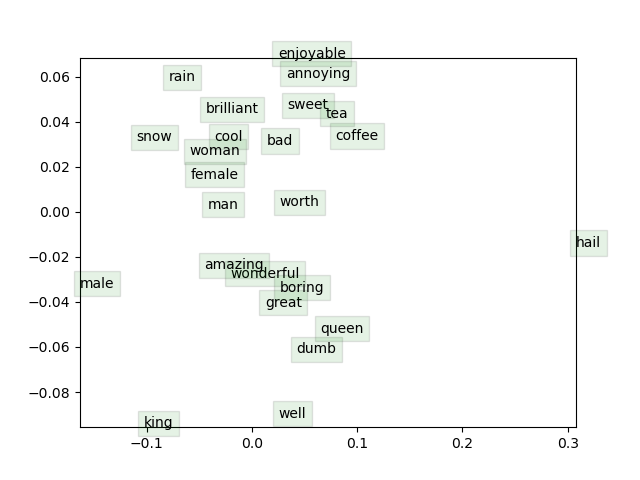
\includegraphics[width=12cm]{word_vectors.png}
    \centering
\end{figure}

In the plot, some synonyms ("amazing", "wonderful", "great") and antonyms (enjoyable, annoying) are cluster together. Terms with similar usage such as ("tea", "coffee"), ("rain", "snow") and ("female", "woman") also group together. Lastly, the linear relationships of word vectors, i.e. vec("king") - vec("male) + vec("female") $\approx$ vec("queen"), is observed.

\end{document}